\chapter{Image Processing}
\label{ch:ImageProcessing}
\graphicspath{{Chapter3/Chapter3Figures/}}
The previous chapter focused on already existing methods of grading tests automatically. It was found that most systems only use image processing, without a machine learning component, to grade these test. In this chapter the core techniques behind processing these answer sheets, using image processing, will be described. By using only these image processing techniques a reasonably accurate system can already be constructed.

For further improvements in accuracy two machine learning approaches will be investigate and implemented. These approaches will be discussed in Chapter \textbf{\ref{ch:MachineLearning}}.

\section{Orientation Detection}

As mentioned in Section \ref{sec:StandardTech} there are two main steps in OMR grading. The first challenge with grading a scanned in answer sheet, is finding the orientation of the template in the image. This can be done by finding five values, including the rotation, offset(xOff,yOff) and a reference point(xRef,yRef). In Chapter \ref{ch:LiteratureStudy} it was determined that the common way to find this orientation is to include specific reference blocks as markers on the page. A disadvantage with this method is that if their is to little markers on the page, the student might accidentally write over them or write something that resembles a marker and confuse the system. The template also looks less attractive if there is many markers. To compensate for this the markers that will be chose, are already present on the template paper. They are the two longest horizontal lines as well as the two vertical lines on the comment box. Together these lines have enough information to determine the rotation, offset and size of the template. The reason these lines are chosen as references, are due to the fact that a Radon transform can easily be applied to determine where they are, as seen in Section \ref{sec:RadonTransform}. But before the orientation of the image can be determined it is a good idea to quickly check if the image might be upside down. This is done to make it easier to find the orientation afterwards. To do this some initial image filtering will be required and will be discussed next.

\subsection{Initial filtering and orientation detection}
\label{sec:InitImageFilter}

To check if and image is upside down the software first needs to find relevant contours on the page. The contours are then filtered out if it does not loosely match the characteristics of a bubble or character block. This is done in 5 steps:

\begin{enumerate}
\item Threshold the image by making all the pixel values either white(lower that the mean) or black(higher that the mean)
\item Do contour analysis on the image to find all the contours, using the python library OpenCV.
\item Filter through the contour array to filter out all contours that are not approximately the size and aspect ratios desired.
\item Save these contours for later use.
\item Determine if more contours lie above the middle of the image(This is true if the image is the right way around). Rotate the image by 180$^{\circ}$ otherwise.
\end{enumerate}

It is important to note that there are still unwanted contours in the list, but for now this list will be sufficient. Once the list is found the software counts the number of contour centerpoints below and above the image center. Figure \ref{fig:reduced} shows the resulting contours found in the image. As can be seen in the figure more bubbles should be below the horizontal center line, for the image to be the right side up. The next step will now be to determine the coordinates of the answers the student wrote down. To do this the template must first be found in the image. This will now be done in Section \ref{sec:RadonTransform}.

\begin{figure}
  \centering
  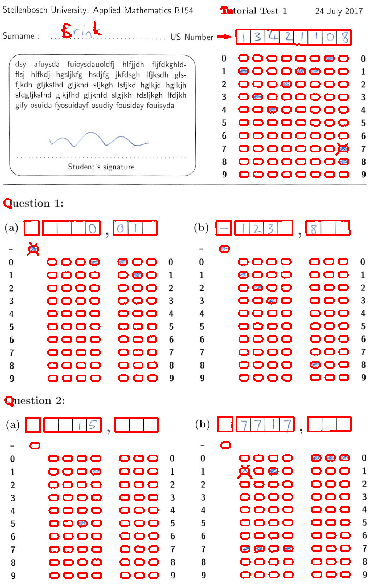
\includegraphics[width=14cm]{Reduced}\\
  \caption{Reduced contours in image.}
  \label{fig:reduced}
\end{figure}

\subsection{Radon Transform}
\label{sec:RadonTransform}

The Radon transform is an integral transform that converts an 2 dimensional image into a 1 dimensional array. An example of this transform can be seen in Figure \ref{fig:RadonT}. This transform is always done over a chosen axis. In this case we will chose the horizontal axis to sum over. By counting up all the pixel values, each in the range 0.0 to 1.0,that corresponds to the same horizontal row a single sum value is calculated. By repeating this process for each row an resulting 1 dimensional array is created. This array provides information about the total pixel concentration on each horizontal line. In the case of the test grader, this can be used to identify where the lines on the pages are, by looking at the maximum values. By slightly rotating the axis over which the Radon transform is calculated new arrays can be calculated. Black lines will cause big values to appear on the Radon transform, when summing parallel with that line. After the correct angle is found the image gets rotated to correct for this angle offset.

\begin{figure}
  \centering
  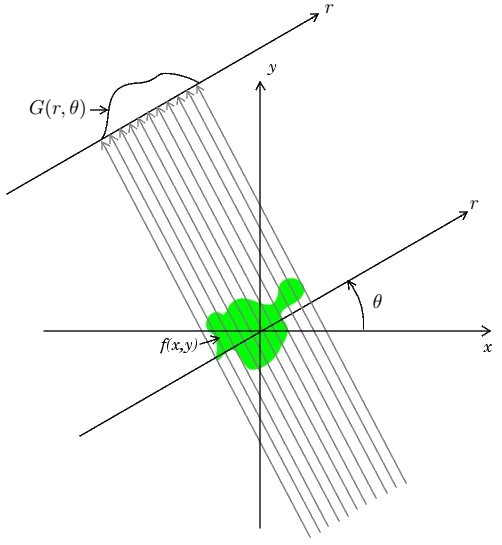
\includegraphics[width=14cm]{RadonT}\\
  \caption{Radon transform applied on a 2 dimensional area, \citet{radon}}
  \label{fig:RadonT}
\end{figure}

\subsection{Finding the template}
\label{sec:findTemplate}

Once the image is rotate correctly the two maximum values of the radon transform will indicate the two horizontal lines in the template. Using those two lines the relative size of the template in the image and y-offset value can be determined . The last step is thus to determine the x-offset value of the template. To do this a vertical Radon transform is applied to detect the two vertical lines of the comment box. This will provide the last x-offset value needed to find the template inside the image as well as additional size evidence to confirm the previously calculated size estimate. Once the template is found the bubble values and digit blocks can be determined, using reference location. These reference locations were calculated in preprocessing done on an empty template. Figure \ref{fig:FinalEstimate} illustrates the final estimation of all the bubbles in the template. The estimated bubble centers are colored red, while the green points represent the centers of all the remaining contours. (Stel dalk beter en duideliker)

\begin{figure}
  \centering
  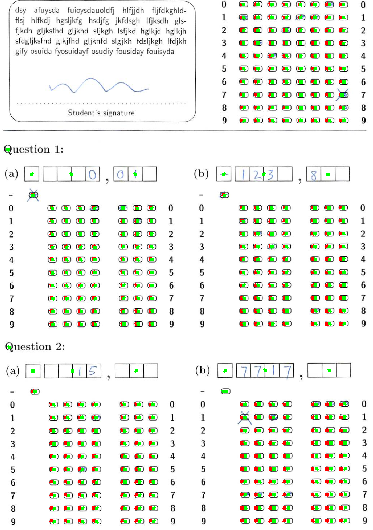
\includegraphics[width=14cm]{FinalEstimate}\\
  \caption{Detection of template in image and estimation of bubble locations.}
  \label{fig:FinalEstimate}
\end{figure}

In Figure \ref{fig:rotate} The final rotation after applying consecutive Radon transforms can be seen.

\begin{figure}
  \centering
  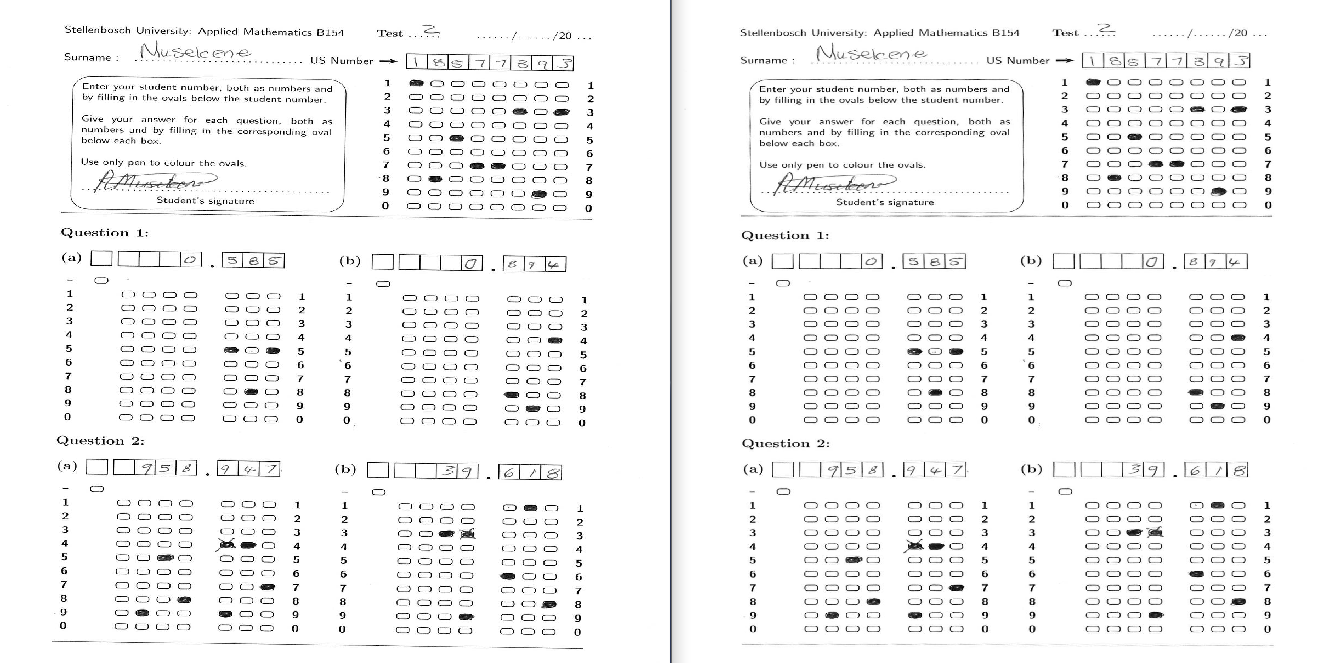
\includegraphics[width=14cm]{Rotation}\\
  \caption{Result in rotation after applying radon transform.}
  \label{fig:rotate}
\end{figure}

In the next step a contour will be assigned to each bubble and then stored.

\section{Bubble detection and processing}

To find the location of each bubble in the image, the system simply takes the contour closest to the estimated bubble location. This can be done in an efficient manner by sorting the contours by there locations. Searching through the contours now becomes linear and of complexity O(n), where n is the number of bubbles. This means that the processing time to find these bubbles is linearly related to the number of bubbles in the template image. Next the data in each contour needs to be processed and stored. The first type of evidence is calculating the average pixel intensity inside the contours. If this value is high the bubble is most likely colored in or crossed out. The advantage of using the closest contour as the bubble's estimated location, over conventional methods now becomes apparent. In conventional methods an estimated area is calculated where the bubble is most likely to be located. This becomes problamatic if the system needs to know if the bubble has been crossed out, as only data about pixel intensities are present. Using contour analisys information about the shape of the bubble entry is also provided. Thus by drawing the smallest possible block around the contour, that still covers every value inside the contour, an area can be calculated. This area will become large when a answer is crossed out, due to the lines stretching outside the initial bubble. By inspecting the area value, the system can successfully determine if the bubble is filled-in and crossed out.

\section{Data processing and grading}

The previous section now allows each bubble to be classified into 3 categories namely, empty, completely filled-in and crossed out. An additional category of partially filled-in will also be introduced, as it aids grading of tests where students write lightly. An algorithm to determine what bubble was chosen can now be described as follows:

\begin{enumerate}
\item Count the number of completely filled-in answers in each column. Store the position of that entry for later use.
\item If there are no completely filled-in answers, count the amount of partially filled-in answers and override the previous values.
\item If the previous result is 0, set the output value for that column to 0.
\item If step 2 or 3 presents a value greater that 1, save the answer sheet to a clashlist to be evaluated manually once the automatic grading of the test are completed.
\end{enumerate}


\section{Conclusion}

This chapter provided an overview of a basic automatic test grading system using image processing and computer vision. The system can achieve acceptable results using only these techniques.

The following chapter will focus on applying additional machine learning techniques to further improve the accuracy of grading these test. Two new test templates will also be introduced. (maak seker jy het daaroor gepraat).